\documentclass[10pt]{article}
\usepackage[utf8]{inputenc}
\usepackage[T1]{fontenc}
\usepackage{amsmath}
\usepackage{amsfonts}
\usepackage{amssymb}
\usepackage[version=4]{mhchem}
\usepackage{stmaryrd}
\usepackage{graphicx}
\usepackage[export]{adjustbox}
\graphicspath{ {./images/} }

\begin{document}
TEST OF MATHEMATICS FOR UNIVERSITY ADMISSION

PAPER 2

Practice paper\\
Additional Materials: Answer sheet

D513/12

Morning

Time: 75 minutes

Please read these instructions carefully, but do not open the question paper until you are told that you may do so.

A separate answer sheet is provided for this paper. Please check you have one. You also require a soft pencil and an eraser.

This paper is the second of two papers.\\
There are 20 questions on this paper. For each question, choose the one answer you consider correct and record your choice on the separate answer sheet. If you make a mistake, erase thoroughly and try again.

There are no penalties for incorrect responses, only points for correct answers, so you should attempt all 20 questions. Each question is worth one mark.

Any rough work should be done on this question paper. No extra paper is allowed.

Please complete the answer sheet with your candidate number, centre number, date of birth, and full name.

Calculators and dictionaries must NOT be used.\\
There is no formulae booklet for this test.

Please wait to be told you may begin before turning this page.

This question paper consists of 18 printed pages and 2 blank pages.

PV3

BLANK PAGE

1 Find the value of

$$
\int_{1}^{2}\left(x^{2}-\frac{4}{x^{2}}\right)^{2} d x
$$

A $\frac{43}{15}$\\
B 3\\
C $\frac{97}{15}$\\
D $\frac{103}{15}$\\
E $\frac{163}{15}$\\
F 18

2

$$
f(x)=\frac{\left(x^{2}+5\right)(2 x)}{\sqrt[4]{x^{3}}}, \quad x>0
$$

Which one of the following is equal to $f^{\prime}(x)$ ?

A $8 x^{\frac{9}{4}}+\frac{40}{3} x^{\frac{1}{4}}$\\
B $\frac{9}{2} x^{\frac{5}{4}}+\frac{5}{2} x^{-\frac{3}{4}}$

C $8 x^{\frac{9}{4}}+\frac{40}{3} x^{-\frac{1}{4}}$

D $\frac{8}{13} x^{\frac{13}{4}}+8 x^{\frac{5}{4}}$

3 What is the value, in radians, of the largest angle $x$ in the range $0 \leq x \leq 2 \pi$ that satisfies the equation $8 \sin ^{2} x+4 \cos ^{2} x=7$ ?

A $\frac{2 \pi}{3}$\\
B $\frac{5 \pi}{6}$\\
C $\frac{4 \pi}{3}$\\
D $\frac{5 \pi}{3}$\\
E $\frac{7 \pi}{4}$\\
F $\frac{11 \pi}{6}$

4 Five sealed urns, labelled P, Q, R, S, and T, each contain the same (non-zero) number of balls. The following statements are attached to the urns.

Urn P This urn contains one or four balls.\\
Urn Q This urn contains two or four balls.\\
Urn R This urn contains more than two balls and fewer than five balls.\\
Urn S This urn contains one or two balls.\\
Urn T This urn contains fewer than three balls.

Exactly one of the urns has a true statement attached to it.\\
Which urn is it?

A Urn P

B Urn Q\\
C Urn R

D Urn S

E Urn T

5 Consider the statement:\\
(\textit{) A whole number $n$ is prime if it is 1 less or 5 less than a multiple of 6 .\\
How many counterexamples to (}) are there in the range $0<n<50$ ?

A 2\\
B 3\\
C 4\\
D 5\\
E 6

6 The sequence of functions $f_{1}(x), f_{2}(x), f_{3}(x), \ldots$ is defined as follows:

$$
\begin{aligned}
f_{1}(x) & =x^{10} \\
f_{n+1}(x) & =x f_{n}^{\prime}(x) \text { for } n \geq 1
\end{aligned}
$$

where $f_{n}^{\prime}(x)=\frac{d f_{n}(x)}{d x}$\\
Find the value of

$$
\sum_{n=1}^{20} f_{n}(x)
$$

A $\frac{x^{10}\left(x^{20}-1\right)}{x-1}$

B $\frac{x^{10}\left(x^{21}-1\right)}{x-1}$\\
C $\left(\frac{10^{20}-1}{9}\right) x^{10}$\\
D $\left(\frac{10^{21}-1}{9}\right) x^{10}$\\
$\mathrm{E} \quad\left(\frac{(10 x)^{20}-1}{10 x-1}\right) x^{10}$\\
$\mathbf{F} \quad\left(\frac{(10 x)^{21}-1}{10 x-1}\right) x^{10}$

G $\quad x^{10}+x^{9}+x^{8}+\cdots+x+1$

H $x^{10}+10 x^{9}+(10 \times 9) x^{8}+\cdots+(10 \times 9 \times \ldots \times 2) x+(10 \times 9 \times \ldots \times 2 \times 1)$

7 The four real numbers $a, b, c$, and $d$ are all greater than 1 .\\
Suppose that they satisfy the equation $\log _{c} d=\left(\log _{a} b\right)^{2}$.\\
Use some of the lines given to construct a proof that, in this case, it follows that

$$
(*) \log _{b} d=\left(\log _{a} b\right)\left(\log _{a} c\right)
$$

(1) Let $x=\log _{a} b$ and $y=\log _{a} c$\\
(2) $d=\left(c^{x}\right)^{2}$\\
(3) $d=c^{\left(x^{2}\right)}$\\
(4) $d=b^{x y}$\\
(5) $d=\left(a^{y}\right)^{\left(x^{2}\right)}$\\
(6) $d=\left(\left(a^{y}\right)^{x}\right)^{2}$\\
(7) $d=\left(a^{x}\right)^{x y}$\\
(8) $d=a^{\left(y^{2 x}\right)}$\\
(9) $d=a^{\left(x^{2} y\right)}$

A (1). Then (2), so (6), so (8), so (7), and therefore (4), hence (\textit{) as required.\\
B (1). Then (2), so (7), so (8), so (6), and therefore (4), hence (}) as required.\\
C (1). Then (3), so (5), so (9), so (7), and therefore (4), hence (\textit{) as required.\\
D (1). Then (3), so (7), so (9), so (5), and therefore (4), hence (}) as required.\\
E (1). Then (4), so (5), so (9), so (7), and therefore (3), hence (\textit{) as required.\\
F (1). Then (4), so (6), so (8), so (7), and therefore (2), hence (}) as required.\\
G (1). Then (4), so (7), so (8), so (6), and therefore (2), hence (\textit{) as required.\\
H (1). Then (4), so (7), so (9), so (5), and therefore (3), hence (}) as required.

8 A region is defined by the inequalities $x+y>6$ and $x-y>-4$\\
Consider the three statements:\\
$1 x>1$\\
$2 y>5$\\
$3(x+y)(x-y)>-24$

Which of the above statements is/are true for every point in the region?

A none\\
B 1 only\\
C 2 only\\
D 3 only\\
E 1 and 2 only\\
F 1 and 3 only\\
G 2 and 3 only\\
H 1, 2 and 3

9 Triangles $A B C$ and $X Y Z$ have the same area.\\
Which of these extra conditions, taken independently, would imply that they are congruent?\\
(1) $A B=X Y$ and $B C=Y Z$\\
(2) $A B=X Y$ and $\angle A B C=\angle X Y Z$\\
(3) $\angle A B C=\angle X Y Z$ and $\angle B C A=\angle Y Z X$

\begin{center}
\begin{tabular}{|l|l|l|l|}
\hline
 & Condition (1) & Condition (2) & Condition (3) \\
\hline
A & Does not imply congruent & Does not imply congruent & Does not imply congruent \\
\hline
B & Does not imply congruent & Does not imply congruent & Implies congruent \\
\hline
C & Does not imply congruent & Implies congruent & Does not imply congruent \\
\hline
D & Does not imply congruent & Implies congruent & Implies congruent \\
\hline
E & Implies congruent & Does not imply congruent & Does not imply congruent \\
\hline
F & Implies congruent & Does not imply congruent & Implies congruent \\
\hline
G & Implies congruent & Implies congruent & Does not imply congruent \\
\hline
H & Implies congruent & Implies congruent & Implies congruent \\
\hline
\end{tabular}
\end{center}

10 In this question $x$ and $y$ are non-zero real numbers.\\
Which one of the following is sufficient to conclude that $x<y$ ?

A $x^{4}<y^{4}$\\
B $y^{4}<x^{4}$\\
C $x^{-1}<y^{-1}$\\
D $y^{-1}<x^{-1}$\\
E $x^{\frac{3}{5}}<y^{\frac{3}{5}}$\\
F $y^{\frac{3}{5}}<x^{\frac{3}{5}}$\\
$11 f(x)$ is a polynomial with real coefficients.\\
The equation $f(x)=0$ has exactly two real roots, $x=-p$ and $x=p$, where $p>0$.\\
Consider the following three statements:\\
$1 \quad f^{\prime}(x)=0$ for exactly one value of $x$ between $-p$ and $p$\\
2 The area between the curve $y=f(x)$, the $x$-axis and the lines $x=-p$ and $x=p$ is given by $2 \int_{0}^{p} f(x) \mathrm{d} x$\\
3 The graph of $y=-f(-x)$ intersects the $x$-axis at the points $x=-p$ and $x=p$ only

Which of the above statements must be true?

A none\\
B 1 only\\
C 2 only\\
D 3 only\\
E 1 and 2 only\\
F 1 and 3 only\\
G 2 and 3 only\\
H 1, 2 and 3

12 The first term of an arithmetic sequence is $a$ and the common difference is $d$.\\
The sum of the first $n$ terms is denoted by $S_{n}$.\\
If $S_{8}>3 S_{6}$, what can be deduced about the sign of $a$ and the sign of $d$ ?

A both $a$ and $d$ are negative\\
B $a$ is positive, $d$ is negative\\
C $\quad a$ is negative, $d$ is positive\\
D $a$ is negative, but the sign of $d$ cannot be deduced\\
E $d$ is negative, but the sign of $a$ cannot be deduced\\
F neither the sign of $a$ nor the sign of $d$ can be deduced

13 In this question, $a, b$, and $c$ are positive integers.\\
The following is an attempted proof of the false statement:\\
If $a$ divides $b c$, then $a$ divides $b$ or $a$ divides $c$.\\[0pt]
[' $a$ divides $b c$ ' means ' $a$ is a factor of $b c$ ']\\
Which line contains the error in this proof?

\begin{enumerate}
  \item The statement is equivalent to if $a$ does not divide $b$ and $a$ does not divide $c$ then $a$ does not divide $b c^{\prime}$.
  \item Suppose $a$ does not divide $b$ and $a$ does not divide $c$. Then the remainder when dividing $b$ by $a$ is $r$, where $0<r<a$, and the remainder when dividing $c$ by $a$ is $s$, where $0<s<a$.
  \item So $b=a x+r$ and $c=a y+s$ for some integers $x$ and $y$.
  \item Thus $b c=a(a x y+x s+y r)+r s$.
  \item So the remainder when dividing $b c$ by $a$ is $r s$.
  \item Since $r>0$ and $s>0$, it follows that $r s>0$.
  \item Hence $a$ does not divide $b c$.
\end{enumerate}

A Line 1\\
B Line 2\\
C Line 3\\
D Line 4\\
E Line 5\\
F Line 6\\
$14 f(x)=a x^{4}+b x^{3}+c x^{2}+d x+e$, where $a, b, c, d$, and $e$ are real numbers.\\
Suppose $f(x)=1$ has $p$ distinct real solutions, $f(x)=2$ has $q$ distinct real solutions, $f(x)=3$ has $r$ distinct real solutions, and $f(x)=4$ has $s$ distinct real solutions.

Which one of the following is not possible?

A $\quad p=1, q=2, r=4$ and $s=3$\\
B $\quad p=1, q=3, r=2$ and $s=4$\\
C $\quad p=1, q=4, r=3$ and $s=2$\\
D $p=2, q=4, r=3$ and $s=1$\\
E $\quad p=4, q=3, r=2$ and $s=1$

15 Consider the quadratic $f(x)=x^{2}-2 p x+q$ and the statement:\\
$\left(^{*}\right) f(x)=0$ has two real roots whose difference is greater than 2 and less than 4.\\
Which one of the following statements is true if and only if (*) is true?

A $q<p^{2}<q+4$

B $\sqrt{q+1}<p<\sqrt{q+4}$

C $\quad q-3 \leq p^{2}-4 \leq q$

D $\quad q<p^{2}-1<q+3$

E $\quad q-2<p^{2}-3<q+2$

16\\
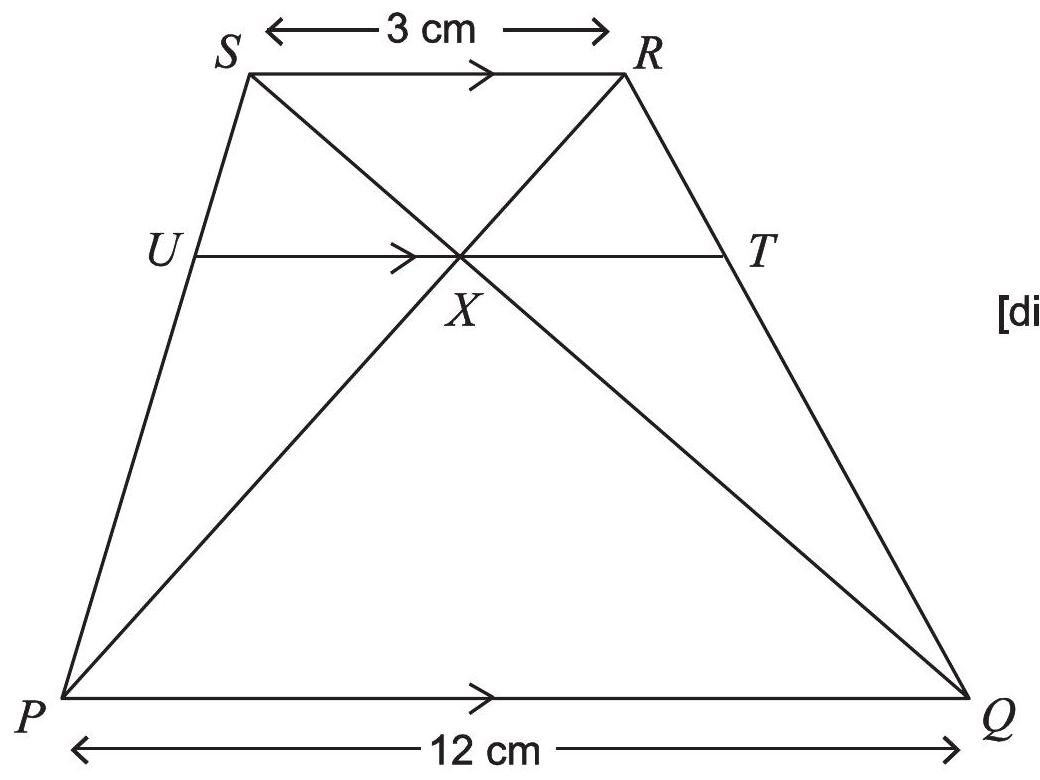
\includegraphics[max width=\textwidth, alt={}, center]{679ccde2-578a-4cd5-962e-a450a2d005a3-15_780_1040_221_283}

In the figure, $P Q R S$ is a trapezium with $P Q$ parallel to $S R$.\\
The diagonals of the trapezium meet at $X$.\\
$U$ lies on $S P$ and $T$ lies on $R Q$ such that $U T$ is a line segment through $X$ parallel to $P Q$.

The length of $P Q$ is 12 cm and the length of $S R$ is 3 cm .\\
What, in centimetres, is the length of UT?

A 4.2\\
B 4.5\\
C 4.8\\
D 5.25\\
E 6

17 Consider these simultaneous equations, where $c$ is a constant:

$$
\begin{aligned}
& y=3 \sin x+2 \\
& y=x+c
\end{aligned}
$$

Which of the following statements is/are true?

1 For some value of $c$ : there is exactly one solution with $0 \leq x \leq \pi$ and there is at least one solution with $-\pi<x<0$.

2 For some value of $c$ : there is exactly one solution with $0 \leq x \leq \pi$ and there are no solutions with $-\pi<x<0$.

3 For some value of $c$ : there is exactly one solution with $0 \leq x \leq \pi$ and there are no solutions with $x>\pi$.

A none\\
B 1 only\\
C 2 only\\
D 3 only\\
E 1 and 2 only\\
F 1 and 3 only\\
G 2 and 3 only\\
H 1, 2 and 3

18 Consider this statement about a function $f(x)$ :\\
$\left(^{*}\right)$ If $(f(x))^{2} \leq 1$ for all $-1 \leq x \leq 1$ then $\int_{-1}^{1}(f(x))^{2} \mathrm{~d} x \leq \int_{-1}^{1} f(x) \mathrm{d} x$ Which one of the following functions provides a counterexample to (*)?

A $f(x)=x+\frac{1}{2}$\\
B $f(x)=x-\frac{1}{2}$\\
C $f(x)=x+x^{3}$

D $f(x)=x-x^{3}$

E $f(x)=x^{2}+x^{4}$

F $f(x)=x^{2}-x^{4}$

19 Some identical unit cubes are used to construct a three-dimensional object by gluing them together face to face.

Sketches of this object are made by looking at it from the right-hand side, from the front and from above. These sketches are called the side elevation, the front elevation, and the plan view respectively.\\
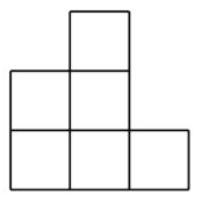
\includegraphics[max width=\textwidth, alt={}, center]{679ccde2-578a-4cd5-962e-a450a2d005a3-18_200_202_575_486}

This is the side elevation of the object.\\
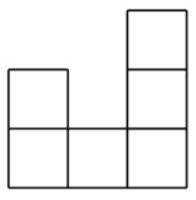
\includegraphics[max width=\textwidth, alt={}, center]{679ccde2-578a-4cd5-962e-a450a2d005a3-18_200_196_794_488}

This is the front elevation of the object.\\
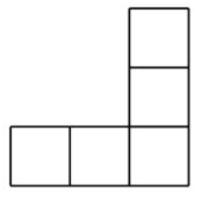
\includegraphics[max width=\textwidth, alt={}, center]{679ccde2-578a-4cd5-962e-a450a2d005a3-18_197_202_1014_486}

This is the plan view of the object.

How many cubes were used to construct the object?

A exactly 6\\
B either 6 or 7\\
C exactly 7\\
D either 7 or 8\\
E exactly 8\\
F either 8 or 9\\
G exactly 9

20 Each interior angle of a regular polygon with $n$ sides is $\frac{3}{4}$ of each interior angle of a second regular polygon with $m$ sides.

How many pairs of positive integers $n$ and $m$ are there for which this statement is true?

A none\\
B 1\\
C 2

D 3\\
E 4\\
F 5\\
G 6\\
H infinitely many

END OF TEST

BLANK PAGE


\end{document}